\documentclass[twocolumn]{article}
\usepackage{amsmath}
\usepackage{epsfig}
\usepackage{psfig}
\usepackage{graphicx}
\usepackage{url}
\usepackage{times}
\usepackage{listings}
\usepackage{multirow}
\usepackage[colorlinks,linkcolor=red,anchorcolor=blue,citecolor=green]{hyperref}
\setlength{\columnsep}{22pt}
\newcommand{\MLR}{Multiple Linear Regression}
\newcommand{\mlr}{multiple linear regression}
\newcommand{\Mlr}{Multiple linear regression}
\lstdefinestyle{rlanguage}{
  belowcaptionskip=1\baselineskip,
  breaklines=true,
  frame=L,
  xleftmargin=\parindent,
  language=R,
  showstringspaces=false,
  basicstyle=\footnotesize\ttfamily,
  numbers=left,
  numbersep=4pt,
  keywordstyle=\bfseries\color{red},
  commentstyle=\itshape\color{gray},
  identifierstyle=\color{blue},
  stringstyle=\color{orange},
}
\begin{document}
\lstset{escapechar=@,style=rlanguage}
\title{Linear Regression Analysis of Bike Sharing System }

\author{Wang Xin\\ \vspace{0.5cm}\\
 10302010023}

\date{}
\maketitle
\begin{abstract}
In this report, we describe a brief process of multiple linear regression for a bike sharing system. We exploit the R language to estimate a linear model of bike sharing counts to multiple predictors and detailed analyses will be given in this report.
The final model suggests a significant relationship between bike sharing counts and predictors given in the input data file like whether conditions and workdays. It is also noteworthy that the resultant model is not the unique answer since the relationship among predictors and outcomes could be explained in more than one mathematical expressions.
\end{abstract}

\section{Introduction}
\label{sec:intro}

\section{Analysis of Techniques}
\label{sec:technique}
\subsection{Introduction to Linear Regression}
In this project, we will use \emph{Multiple Linear Regression} to provide a model that predicts bike rentals, based on given values pf the specified predictors.

Simple Linear Regression is a common method for predicting a quantitative response Y based on the predictor variable X. We usually assume that there is an approximatively linear relation between X and Y, which could be expressed as Equation~\ref{equ:simple}
\begin{equation}\label{equ:simple}
  Y \approx \beta_0+\beta_1X
\end{equation}
In this equation $\beta_0$ is the intercept and $\beta_1$ is the slope. Both $\beta_0$ and $\beta_1$ are the \emph{coefficients} or \emph{parameters} of the model.
Once we have used the training data to calculate the parameter $\beta_0$ and $\beta_1$, we can predict the future response by calculating: $\hat{y} = \hat{\beta_0} + \hat{\beta_1}x$, where $\hat{y}$ is a prediction of Y based on a predictor value X = x. $\hat{\beta}$ is an estimated value for an unknown parameter, likewise, $\hat{y}$ is a predicted response.

The case of one explanatory variable is called simple linear regression. For more than one explanatory variable, the process is called \mlr. In this report, there are more than ten predictors possibly related to the final response, thus we should apply {\mlr} to construct the model.

{\Mlr} is an extension of the simple linear regression model. A typical expression of {\mlr} containing \textit{p} predictors is shown as Equation~\ref{equ:mlr}.
\begin{equation}\label{equ:mlr}
  Y = \beta_0 + \beta_1X_1 + \beta_2X_2 + ... + \beta_pX_p + \epsilon
\end{equation}
In this equation $X_j$ represents the $j^{th}$ predictor and $\beta_j$ is the association between the $j^{th}$ variable and the response. It indicates the average effect on Y of a one unit increase on $X_j$, holding all other predictors fixed.

We use a least square approach to estimate the regression coefficients and this means we have to minimize the \emph{Residual Sum of Square (RSS)}, which is calculated by Equation~\ref{equ:rss}.

\begin{multline}
\label{equ:rss}
  RSS = \sum_{i = 1}^{n}{e_i^2} = \sum_{i = 1}^{n}{(y_i - \hat{y}_i)}\\
   = \sum_{i = 1}^{n}{(y_i - \hat{\beta}_0 - \hat{\beta}_1x_{i1} - \hat{\beta}_1x_{i2} - ... - \hat{\beta}_px_{ip})^2}
\end{multline}

Generally speaking, there are four issues to consider when adopting the {\mlr}.
\begin{itemize}
  \item \textbf{Relationship between Response and Predictors}. Like in simple linear regression, we perform the hypothesis test by computing the F-statistic as shown in Equation~\ref{equ:ftest}.
      \begin{multline}\label{equ:ftest}
        F = \frac{(TSS - RSS)/p}{RSS/(n - p - 1)}\\
        \text{TSS = Total Sum of Squares = $\sum{(y_i - \bar{y})^2}$}\\
        \text{RSS = Residual Sum of Squares = $\sum{(y_i - \hat{y_i})^2}$}
      \end{multline}
      If the null hypothesis is true (no relationship between response and predictors), F-statistics $\approx$ 1. Otherwise if the alternative hypothesis is true, F-statistic $\gg$ 1.
  \item \textbf{Deciding on Important Variables}. Best way would be to try out all models with all possible combinations of predictors (all subsets regression). we could decide which combination is best through adjusted $R^2$ or residual plots. There are three practical methods for feature selection: \emph{Forward Selection}, \emph{Backward Selection} and \emph{Mixed Selection}.
  \item \textbf{Model Fit}. We have seen two good measures: RSE and $R^2$; They are both important to judge how well the model fits the data.
  \item \textbf{Predictions}. In {\mlr}, the coefficients $\hat{\beta_0}, \hat{\beta_1},...,\hat{\beta_p}$ are used to define the \emph{least squares plane} as in the following equation:
      \begin{equation}\label{equ:plane}
        \hat{Y} = \hat{\beta_0} = \hat{\beta_1}X_1 + ... + \hat{\beta_p}X_p
      \end{equation}
      In order to understand how certain our estimation is, we can establish a \emph{Confidence Interval}, which tells us the average value of response for chosen values of X. Moreover, in order to answer where a single new observation will fall, we can establish the \emph{Prediction Interval}, which captures a single new random observation, rather than the average observation. It will always be wider than the confidence interval.
\end{itemize}

\subsection{Strengths and Weaknesses}

{\MLR} is a simple but effective method to depict the linear relationship between predictors and responses. R language facilitates us to generate a detailed summary about the regression. From the summary we could understand more about the quality of our estimation.

However, there are also some noteworthy weaknesses about {\mlr}, which lower the precision of linear model .
\begin{itemize}
  \item \textbf{Qualitative Predictors}. Not all predictors in a linear model are \emph{quantitative}, often some predictors will be \emph{qualitative}. We could create dummy variables to depict the qualitative predictors. For qualitative predictors with more than two levels, we could add the number of dummy variables to represent difference levels.
  \item \textbf{Non-linear Relationships between Predictors}. When applying linear regression, we make two very important restrictive assumptions: the relationship between the predictors and response is \emph{additive} and \emph{linear}.
      But in some cases, the true relationship between the response and the predictors may be non-linear. Here we present a very simple way to directly extend the linear model to accommodate non-linear relationships, using \emph{polynomial regression}.
  \item \textbf{Outliers}. An outlier is a point with an unusual response value. Outliers can occur for a variety of reasons: faulty sample, error during data collection, etc.
\end{itemize}


\section{Analysis of Database}
\label{sec:database}

\section{Analysis of Outcomes}
\label{sec:outcome}
\subsection{Data Manipulation}
\subsubsection{Preprocessing}
Before we get down to read all data into our workbench in R, we need to preprocess the file format so as to delete some redundant data and adjust the format of some fields. Generally, out preprocessing includes the following steps:
\begin{itemize}
  \item \textbf{Delete Redundant Data}. For instances, the field \texttt{instant} in  Table~\ref{tab:fields} only records the indexes of data entries, which should be eliminated from the data manipulation.
  \item \textbf{Format Transformation}. The data format of some fields should be transformed, especially some \emph{qualitative} fields such as \texttt{weathersit} and \texttt{holiday}, so that R language could recognize them as qualitative variables and create dummy variables. 
\end{itemize}

We use a simple python script to preprocess the input file, which is provided in Section~\ref{apd:pre} in appendix. After preprocessing, there are totally 15 variables left in the model, the deleted ones are labeled as {\color{red}red} and the transformed ones are labeled as {\color{green}green} in Table~\ref{tab:fields}.

\subsubsection{Fit all Linear Variables}

In the remaining 15 variables, we first fit all predictors in linear form and the response is \texttt{cnt}:
\begin{lstlisting}[style=rlanguage]
>lm.fit_all = lm(cnt~.-registered-casual,data=bicycle)
>summary{lm.fit_all}

Call:
lm(formula = cnt ~ . - registered - casual, data = bicycle)

Residuals:
    Min      1Q  Median      3Q     Max
-396.57  -60.52   -7.94   51.34  440.09

Coefficients:
               Estimate Std. Error t value Pr(>|t|)
(Intercept)    -50.9441     8.9203  -5.711 1.14e-08 ***
seasonSpring   -32.0083     5.7453  -5.571 2.57e-08 ***
seasonSummer     6.2138     4.9737   1.249  0.21156
seasonWinter    35.9871     5.1574   6.978 3.11e-12 ***
.....
---
Signif. codes:  0 ‘***’ 0.001 ‘**’ 0.01 ‘*’ 0.05 ‘.’ 0.1 ‘ ’ 1

Residual standard error: 101.7 on 17330 degrees of freedom
Multiple R-squared:  0.6863,	Adjusted R-squared:  0.6855
F-statistic:   790 on 48 and 17330 DF,  p-value: < 2.2e-16
\end{lstlisting}
From the summary we could see that R language has calculated the slope and intercept for all input linear predictors, besides, it also creates dummy variables for qualitative predictors like \texttt{seasonSpring}, \texttt{seasonSummer}. For detailed information about dummy variables, we can use \texttt{Contrasts} function.

\begin{lstlisting}[style=rlanguage]
> contrasts(season)
       Spring Summer Winter
Autumn      0      0      0
Spring      1      0      0
Summer      0      1      0
Winter      0      0      1
\end{lstlisting}

The result shows that $F-statistic = 729.1$ and $p-value < 2.2e-16$ thus there \textbf{is} a relationship between the predictors and the response \texttt{cnt}. 



\subsection{Graphs and Tables} 

\section{Suggested Model}
\label{sec:model}

Finally, we exploit {\mlr} to generate regression model for three responses \texttt{casual,registered,cnt}. The results are shown as follows.

\subsection{Cnt}
\begin{lstlisting}[style=rlanguage]
Call:
lm(formula = cnt ~ season + yr + mnth + hr + holiday + weekday +
    weathersit + (temp + hum + windspeed)^2 + poly(hum, 4) +
    I(windspeed^2), data = bicycle)

Residuals:
    Min      1Q  Median      3Q     Max
-366.40  -59.41   -5.70   50.19  424.33

Coefficients: (1 not defined because of singularities)
               Estimate Std. Error t value Pr(>|t|)
(Intercept)    -150.337     13.187 -11.400  < 2e-16 ***
seasonSpring    -31.664      5.699  -5.556 2.80e-08 ***
seasonSummer      8.979      4.925   1.823  0.06831 .
seasonWinter     35.209      5.115   6.883 6.06e-12 ***
yry1             84.671      1.559  54.324  < 2e-16 ***
...
weathersitMist   -9.529      1.909  -4.992 6.02e-07 ***
weathersitRain  -83.097     58.292  -1.426  0.15403
weathersitSnow  -60.884      3.387 -17.976  < 2e-16 ***
temp            380.473     19.070  19.951  < 2e-16 ***
hum             114.093     14.960   7.626 2.54e-14 ***
windspeed        85.546     36.478   2.345  0.01903 *
poly(hum, 4)1        NA         NA      NA       NA
poly(hum, 4)2  -989.456    113.454  -8.721  < 2e-16 ***
poly(hum, 4)3   289.732    103.030   2.812  0.00493 **
poly(hum, 4)4   274.210    104.049   2.635  0.00841 **
I(windspeed^2) -215.503     36.334  -5.931 3.07e-09 ***
temp:hum       -340.669     24.058 -14.161  < 2e-16 ***
temp:windspeed  190.288     35.142   5.415 6.21e-08 ***
hum:windspeed  -181.499     35.112  -5.169 2.38e-07 ***
---
Signif. codes:  0 ‘***’ 0.001 ‘**’ 0.01 ‘*’ 0.05 ‘.’ 0.1 ‘ ’ 1

Residual standard error: 100.6 on 17320 degrees of freedom
Multiple R-squared:  0.6933,	Adjusted R-squared:  0.6923
F-statistic: 675.1 on 58 and 17320 DF,  p-value: < 2.2e-16
\end{lstlisting}

\subsection{Casual}
\begin{lstlisting}[style = rlanguage]
> lm.fit_fin = lm(casual~season+yr+mnth+hr+holiday+weekday+weathersit+(temp+hum+windspeed)^2+poly(hum,4)+I(windspeed^2),data=bicycle)
> summary(lm.fit_fin)

Call:
lm(formula = casual ~ season + yr + mnth + hr + holiday + weekday +
    weathersit + (temp + hum + windspeed)^2 + poly(hum, 4) +
    I(windspeed^2), data = bicycle)

Residuals:
    Min      1Q  Median      3Q     Max
-91.485 -18.393  -3.001  12.852 251.042

Coefficients: (1 not defined because of singularities)
                Estimate Std. Error t value Pr(>|t|)
(Intercept)     -36.9387     4.0705  -9.075  < 2e-16 ***
seasonSpring     -1.5635     1.7591  -0.889 0.374127
seasonSummer      9.0139     1.5203   5.929 3.10e-09 ***
seasonWinter      0.4354     1.5790   0.276 0.782745
yry1             11.6976     0.4811  24.314  < 2e-16 ***
...
temp            158.5548     5.8865  26.935  < 2e-16 ***
hum              50.0185     4.6179  10.831  < 2e-16 ***
windspeed        -5.3359    11.2598  -0.474 0.635584
poly(hum, 4)1         NA         NA      NA       NA
poly(hum, 4)2  -218.2046    35.0205  -6.231 4.75e-10 ***
poly(hum, 4)3    82.0113    31.8030   2.579 0.009925 **
poly(hum, 4)4   101.5730    32.1174   3.163 0.001567 **
I(windspeed^2)  -53.8757    11.2155  -4.804 1.57e-06 ***
temp:hum       -152.3517     7.4260 -20.516  < 2e-16 ***
temp:windspeed   72.3110    10.8474   6.666 2.70e-11 ***
hum:windspeed   -31.4267    10.8382  -2.900 0.003741 **
---
Signif. codes:  0 ‘***’ 0.001 ‘**’ 0.01 ‘*’ 0.05 ‘.’ 0.1 ‘ ’ 1

Residual standard error: 31.06 on 17320 degrees of freedom
Multiple R-squared:  0.6045,	Adjusted R-squared:  0.6032
F-statistic: 456.5 on 58 and 17320 DF,  p-value: < 2.2e-16
\end{lstlisting}

\subsection{Registered}
\begin{lstlisting}[style=rlanguage]
> lm.fit_fin = lm(registered~season+yr+mnth+hr+holiday+weekday+weathersit+(temp+hum+windspeed)^2+poly(hum,4)+I(windspeed^2),data=bicycle)
> summary(lm.fit_fin)

Call:
lm(formula = registered ~ season + yr + mnth + hr + holiday +
    weekday + weathersit + (temp + hum + windspeed)^2 + poly(hum,
    4) + I(windspeed^2), data = bicycle)

Residuals:
    Min      1Q  Median      3Q     Max
-346.74  -48.33   -4.84   45.05  409.22

Coefficients: (1 not defined because of singularities)
                 Estimate Std. Error t value Pr(>|t|)
(Intercept)    -113.39857   11.12982 -10.189  < 2e-16 ***
seasonSpring    -30.10083    4.80975  -6.258 3.98e-10 ***
seasonSummer     -0.03502    4.15677  -0.008 0.993279
seasonWinter     34.77392    4.31732   8.055 8.49e-16 ***
yry1             72.97351    1.31547  55.473  < 2e-16 ***
...
I(windspeed^2) -161.62695   30.66584  -5.271 1.38e-07 ***
temp:hum       -188.31749   20.30450  -9.275  < 2e-16 ***
temp:windspeed  117.97659   29.65931   3.978 6.99e-05 ***
hum:windspeed  -150.07255   29.63427  -5.064 4.14e-07 ***
---
Signif. codes:  0 ‘***’ 0.001 ‘**’ 0.01 ‘*’ 0.05 ‘.’ 0.1 ‘ ’ 1

Residual standard error: 84.92 on 17320 degrees of freedom
Multiple R-squared:  0.6863,	Adjusted R-squared:  0.6852
F-statistic: 653.2 on 58 and 17320 DF,  p-value: < 2.2e-16
\end{lstlisting}

\subsection{Graphs}
Here we present the residual graph for all the three predictors. From the following three graphs we could observe that there are no explicit patterns in \texttt{Residual vs Fitted} graph, indicating that a linear model could describe the relationship between predictors and response well. Moreover, most points in \texttt{Normal Q-Q} graph locates near the line with the slope of 45 degree thus the standardized residuals obeys to a normal distribution with $\sigma = 0$, which means that the normality hypothesis holds.

\begin{figure}[ht]
  \centering
  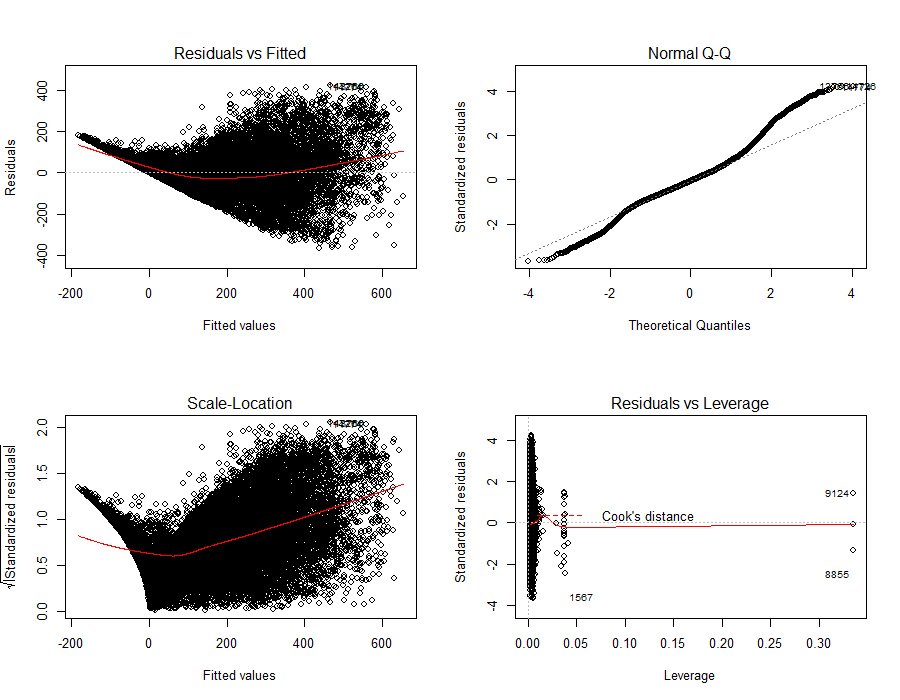
\includegraphics[width=\linewidth]{pic/cnt.png}\\
  \caption{Residual Graphs about Response \texttt{cnt}}\label{fig:cnt}
\end{figure}

\begin{figure}[ht]
  \centering
  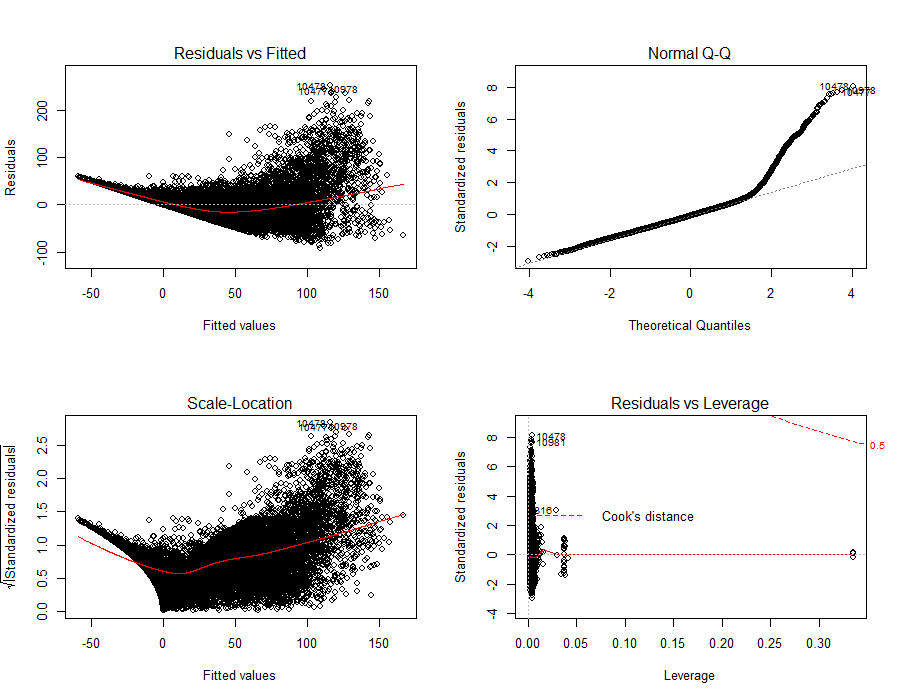
\includegraphics[width=\linewidth]{pic/casual.png}\\
  \caption{Residual Graphs about Response \texttt{casual}}\label{fig:casual}
\end{figure}

\begin{figure}[ht]
  \centering
  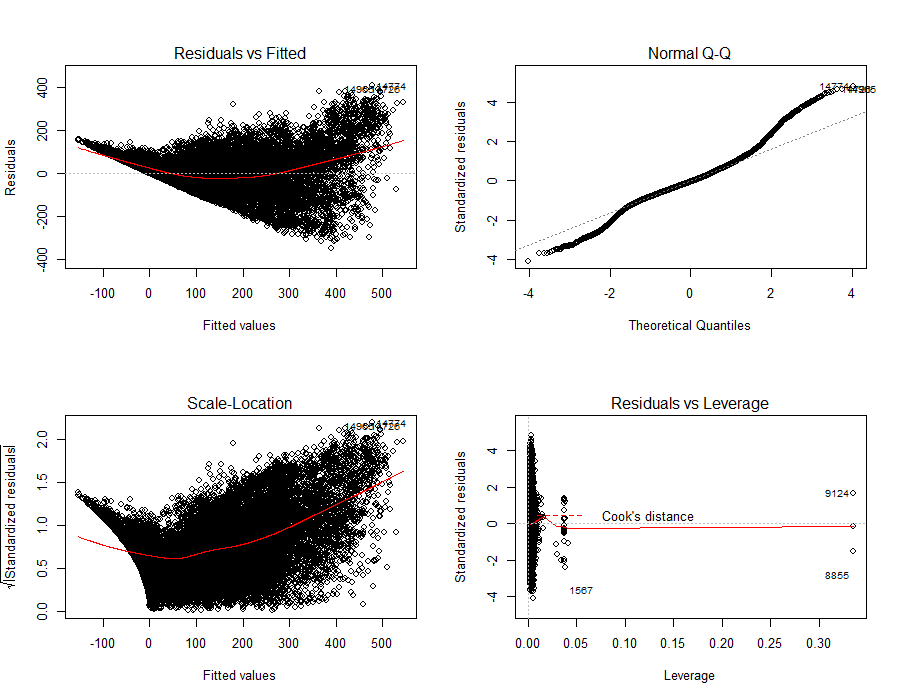
\includegraphics[width=\linewidth]{pic/registered.png}\\
  \caption{Residual Graphs about Response \texttt{registered}}\label{fig:registered}
\end{figure}

\subsection{Questions}
Now we could answer the seven important questions.
\begin{enumerate}
  \item \textit{Is there a relationship between predictors and responses?}\\
   We first set the null hypothesis, $H_0 = \beta_0 = \beta_1 = ... = \beta_p = 0$. Then we compute the F-statistic, which tells us if we should reject the null hypothesis:
      \\$F-statistic$ = 456.5 on 58 and 17320 DF  \\$p-value <$ 2.2e-16\\
   A high F-statistic and low p-value indicate clear evidence between predictors and responses.

  \item \textit{How strong is the relationship between predictors and responses?}\\
      We compute two measures: RSE and $R^2$.\\
       RSE (Residual Standard Error): standard deviation of the response from the population regression line;
       \begin{equation}\label{equ:rse}
         RSE = \sqrt{\frac{1}{n-p-1}RSS}
       \end{equation}
        $R^2$: percentage of variability in the response that is explained by the predictors.
        \begin{equation}\label{equ:rsq}
        R^2 = \frac{TSS-RSS}{TSS} = 1-\frac{RSS}{TSS}
       \end{equation}
       Taking \texttt{registered} as an example, RSE = 84.92 and $R^2$ = 0.6852, thus almost 70\% of variance in \texttt{registered} is explained by the predictors.
  \item \textit{Which predictors contribute to responses?}\\
      From the summary  in Section~\ref{sec:fitall} we could find that after data transformation, all predictors except \texttt{atemp} and \texttt{workingday} contribute to the responses.
  \item \textit{ How accurately can we estimate the effect of each predictor on responses?}\\
      We can use \texttt{confint} function to construct 95\% confidence intervals $(2 \times SE(\hat{\beta_i})$ for each $X_i$).
      \begin{lstlisting}[style=rlanguage]
> confint(lm.fit_reg)
                       2.5 %        97.5 %
(Intercept)    -135.21414187  -91.58299531
seasonSpring    -39.52842681  -20.67323457
seasonSummer     -8.18271186    8.11267767
seasonWinter     26.31153938   43.23629561
...
poly(hum, 4)4     0.50778077  344.76708025
I(windspeed^2) -221.73508938 -101.51881134
temp:hum       -228.11636613 -148.51860843
temp:windspeed   59.84134008  176.11184295
hum:windspeed  -208.15871196  -91.98639067
\end{lstlisting}
  \item \textit{How accurately can we predict future responses?}\\
      To predict an \emph{individual response}, $Y = f(X) + \epsilon$, we can calculate prediction interval.
\begin{lstlisting}[style = rlanguage]
>predict(lm.fit_reg,data.frame(season="Spring",yr = "y0",mnth ="m2", holiday = "No", hr = "h10",weekday = "w5", weathersit="Clear",temp = 0.24, atemp = 0.2879,hum=0.80,windspeed = 0.2),interval="prediction")
      fit       lwr      upr
1 40.1079 -126.6063 206.8221
\end{lstlisting}
Thus 95\% \textbf{Prediction Interval} is [-126.6063, 206.8221].\\
To predict an \emph{average response}, $f(X)$, we can calculate confidence interval.
\begin{lstlisting}[style = rlanguage]
> predict(lm.fit_reg,data.frame(season="Spring",yr = "y0",mnth ="m2", holiday = "No", hr = "h10",weekday = "w5", weathersit="Clear",temp = 0.24, atemp = 0.2879,hum=0.80,windspeed = 0.2),interval="confidence")
      fit      lwr      upr
1 40.1079 30.76016 49.45563
\end{lstlisting}
Thus 95\% \textbf{Confidence Interval} is [30.76016, 49.45563].
  \item \textit{Is the relationship linear?}\\
  Not all predictors are linear according to our analysis in Section~\ref{sec:non-linear}, therefore we transform some predictors to accommodate non-linear relationships.
  \item \textit{ Is there synergy among the predictors?}\\
  Based on the analysis in Section~\ref{sec:interactive}, between many pairs of predictors there are strong interactions such as \texttt{temp:hum} with $p-value < 2e-16$.
      
\end{enumerate}


\appendix

\section{R commands}

\end{document}

